\documentclass[compress,11pt,xcolor=svgnames,aspectratio=169]{beamer}
\usetheme{Esiwace}
\usefonttheme[onlysmall]{structurebold}

%\usepackage{caption}
%\captionsetup{labelformat=empty, format=plain, labelsep=none,textfont=footnotesize}

\usepackage[utf8]{inputenc}
\usepackage[english]{babel}
\usepackage[T1]{fontenc}
\usepackage{eurosym}
\usepackage{ulem}
\usepackage{listings}
\usepackage{ragged2e}  %For \justify and \justifying, but it's not working
\usepackage{pgfgantt}
\usepackage{comment}

\newcommand{\sectionIntro}{
\begin{frame}{Outline}
  \tableofcontents[currentsection,hideothersubsections]%,subsectionstyle=hide/hide/hide
\end{frame}
}

\newcommand{\sectionIntroHidden}{
\begin{frame}{Outline}
  \tableofcontents[currentsection,subsectionstyle=hide/hide/hide]
\end{frame}
}

\makeatletter
\renewcommand{\itemize}[1][]{%
  \beamer@ifempty{#1}{}{\def\beamer@defaultospec{#1}}%
  \ifnum \@itemdepth >2\relax\@toodeep\else
    \advance\@itemdepth\@ne
    \beamer@computepref\@itemdepth% sets \beameritemnestingprefix
    \usebeamerfont{itemize/enumerate \beameritemnestingprefix body}%
    \usebeamercolor[fg]{itemize/enumerate \beameritemnestingprefix body}%
    \usebeamertemplate{itemize/enumerate \beameritemnestingprefix body begin}%
    \list
      {\usebeamertemplate{itemize \beameritemnestingprefix item}}
      {\def\makelabel##1{%
          {%
            \hss\llap{{%
                \usebeamerfont*{itemize \beameritemnestingprefix item}%
                \usebeamercolor[fg]{itemize \beameritemnestingprefix item}##1}}%
          }%
        }%
      }
  \fi%
  \beamer@cramped%
  \justifying% NEW
  %\raggedright% ORIGINAL
  \beamer@firstlineitemizeunskip%
}
\makeatother

\tcbuselibrary{raster}

\DeclareGraphicsExtensions{.pdf,.png,.jpg,}
\graphicspath{{./fig/}}

\title[Summer School -- Input/Output and Middleware]{Summer School on Effective HPC for Climate and Weather \\[0.5cm] Input/Output and Middleware}
\author[Pedro, Kunkel]{Luciana Pedro, Julian Kunkel
}
\institute[WP4 Team]{Department of Computer Science, University of Reading}
\date{18 June 2020}

\begin{document}

%%%%%%%%%%%%%%%%%%%%%%%%%%%%%%%%%%%%%%%%%%%%%%%%%%%%%%%%%%%%
\begin{frame}[plain]
    \titlepage
\end{frame}

%%%%%%%%%%%%%%%%%%%%%%%%%%%%%%%%%%%%%%%%%%%%%%%%%%%%%%%%%%%%
\begin{withoutheadline}
\begin{frame}{Outline}
    \begin{centering}
    \tableofcontents[hideallsubsections]
    \end{centering}

    \disclaimer
\end{frame}
\end{withoutheadline}

% Input/Output and Middleware
% Climate and weather research is typically data-intensive and applications must utilise input/output efficiently. Often, a user struggles to assess observed performance leading to superflux attempts to tune the application and optimise performance in a wrong layer of the stack. The content of this session is twofold. Firstly, we discuss storage layers focusing on the NetCDF middleware and provide a performance model that aids users to identify inefficient I/O. Secondly, we introduce the NetCDF Climate and Forecast (CF) conventions that are often used as a standard to exchange data.

\begin{frame}[t]{Learning Objectives}

\begin{itemize}
\setlength\itemsep{0.4cm}
  \item Describe the role of middleware and file formats (Section Middleware)
  \item Discuss challenges for data-driven research (Section Data)
  \item Identify typical I/O performance issues and their causes (Section Performance)
  \item Apply performance models to assess and optimize the application I/O performance (Section Model)
  \item Design a data model for NetCDF/CF (Section NetCDF)
  \item Describe ongoing research activities in high-performance storage (Section Storage)
\end{itemize}

\end{frame}

\section{Introduction}
\sectionIntro

\subsection{Bottleneck}

\begin{frame}[t]{I/O Bottleneck -- Example}

\begin{center}
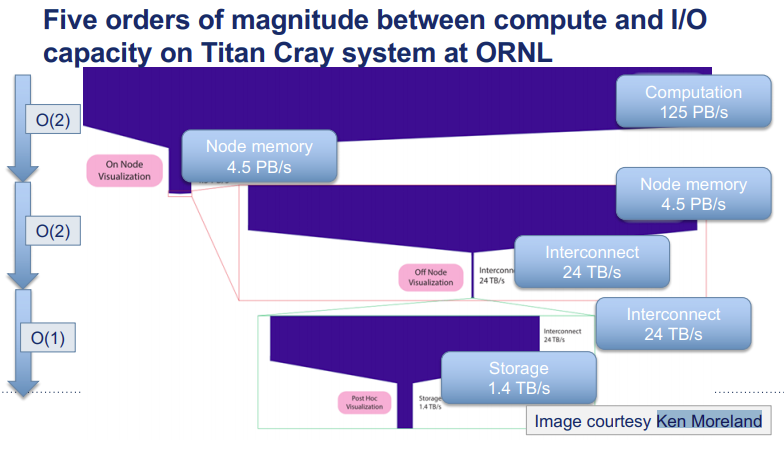
\includegraphics[scale=0.5]{fig/bottleneck-titan}
\end{center}

\end{frame}

\begin{frame}[t]{I/O Bottleneck -- Historical Data}

Kunkel et al. [105] analyze historical data from the German Climate Computing Center (DKRZ) and predict processor performance growth by 20x each generation ($\sim$5 years), while storage throughput/capacity improves by just 6x.

\begin{center}
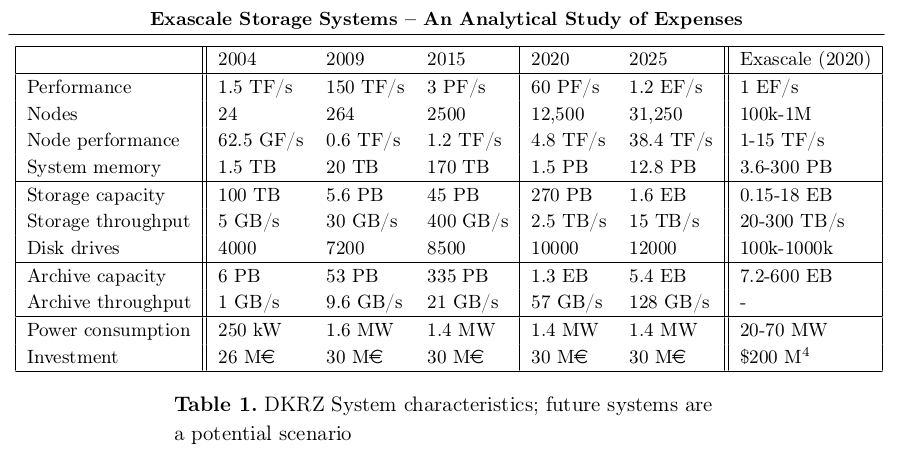
\includegraphics[scale=0.4]{fig/bottleneck-dkrz}
\end{center}

\end{frame}

\subsection{Input/Output}

\begin{frame}[t]{Input/Output}

Input/Output (I/O) is simply data migration.

\begin{itemize}
  \item Memory $\Leftrightarrow$ Disk
\end{itemize}

I/O is a very expensive operation.

\begin{itemize}
  \item Interactions with data in memory and on disk.
\end{itemize}

How is I/O performed?

\begin{itemize}

  \item I/O Pattern

  \begin{itemize}
    \item Number of processes and files.
    \item Characteristics of file access.
  \end{itemize}

\end{itemize}

Where is I/O performed?

\begin{itemize}
  \item Characteristics of the computational system.
  \item Characteristics of the file system.
\end{itemize}

\end{frame}

\begin{frame}[t]{I/O Performance}

\begin{itemize}
\setlength\itemsep{0.4cm}

  \item There is no ``One Size Fits All'' solution to the I/O problem.

  \item Many I/O patterns work well for some range of parameters.

  \item Bottlenecks in performance can occur in many locations.

  \begin{itemize}
    \item Application and/or file system.
  \end{itemize}

  \item Going to extremes with an I/O pattern will typically lead to problems.

  \item Increase performance by decreasing number of I/O operations (latency) and increasing size (bandwidth).

\end{itemize}

\end{frame}

\begin{frame}[t]{I/O Types}

\begin{center}
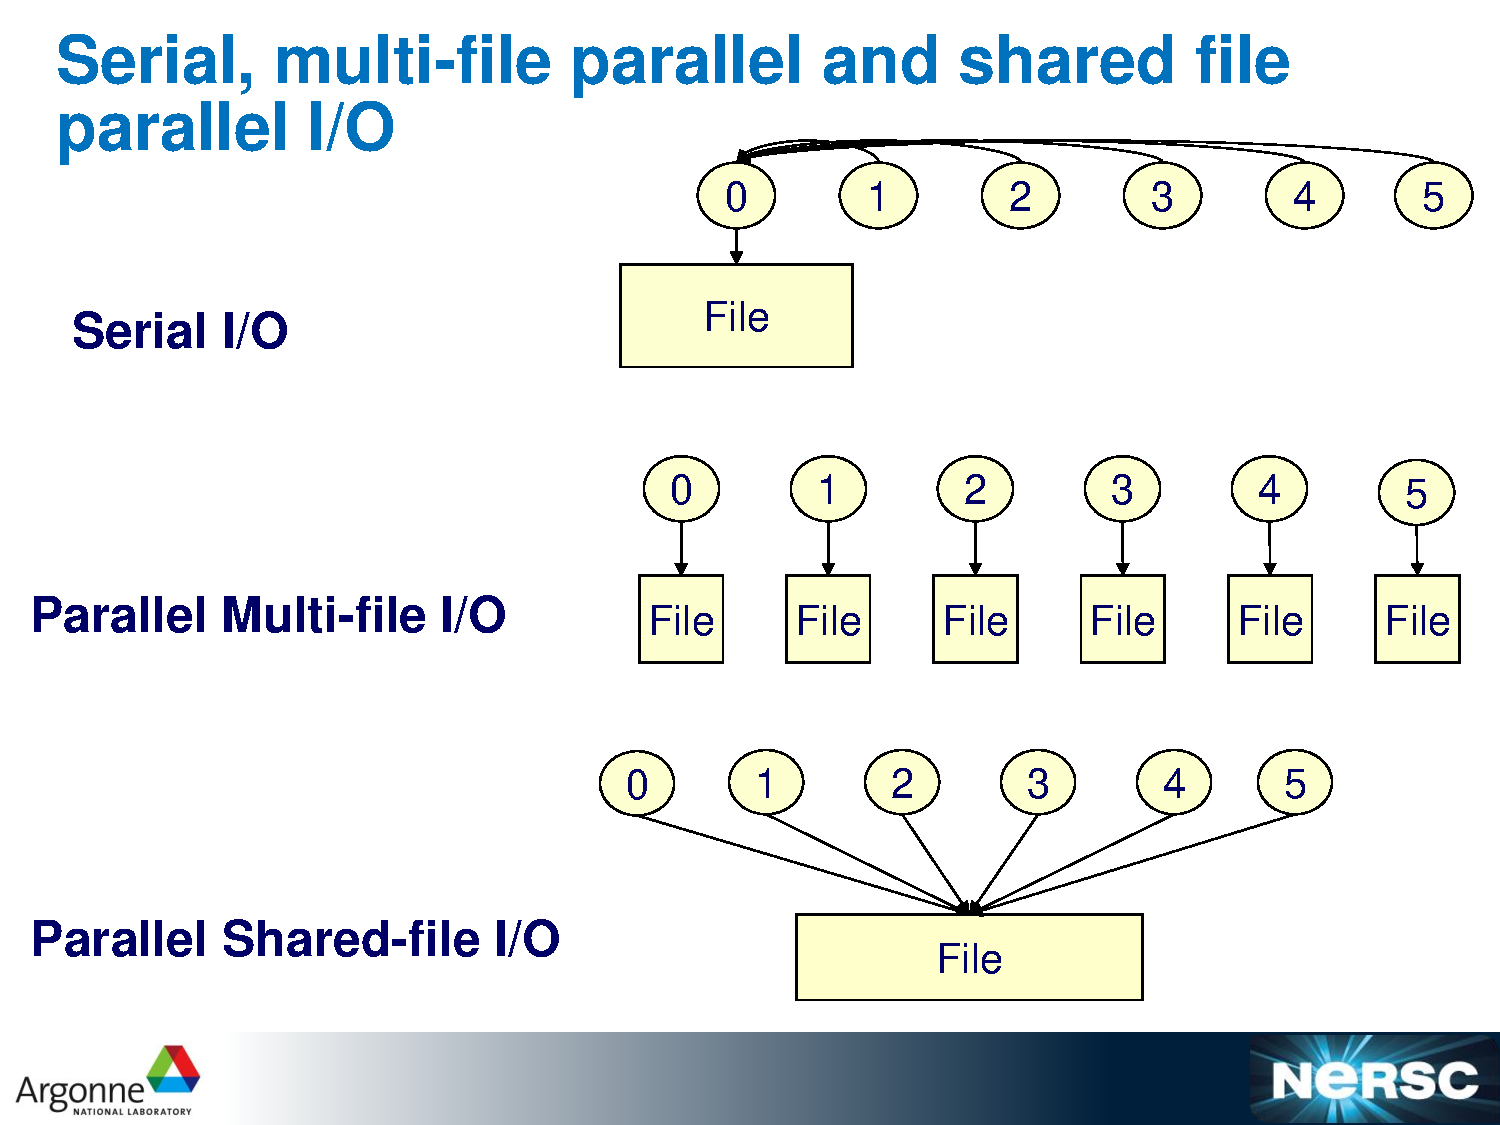
\includegraphics[scale=0.3]{io-types}
\end{center}

\end{frame}

\begin{frame}[t]{I/O Patterns}

\begin{center}
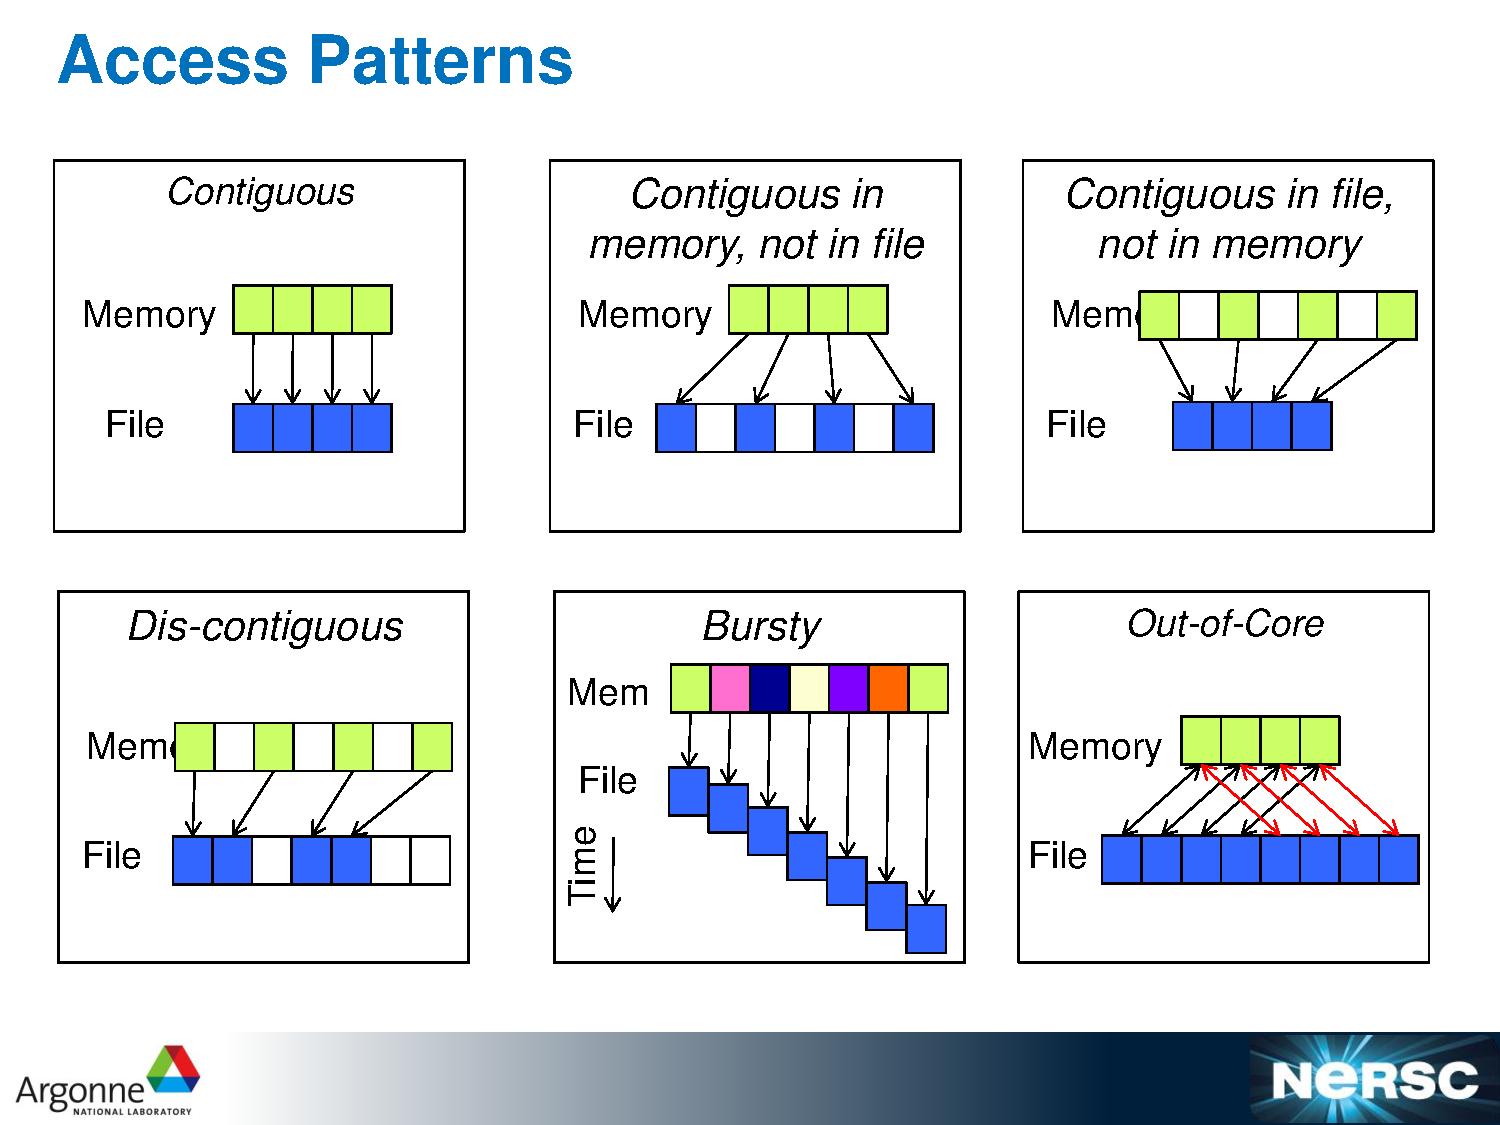
\includegraphics[scale=0.3]{io-patterns}
\end{center}

\end{frame}

\begin{frame}[t]{I/O Probs}

\begin{center}
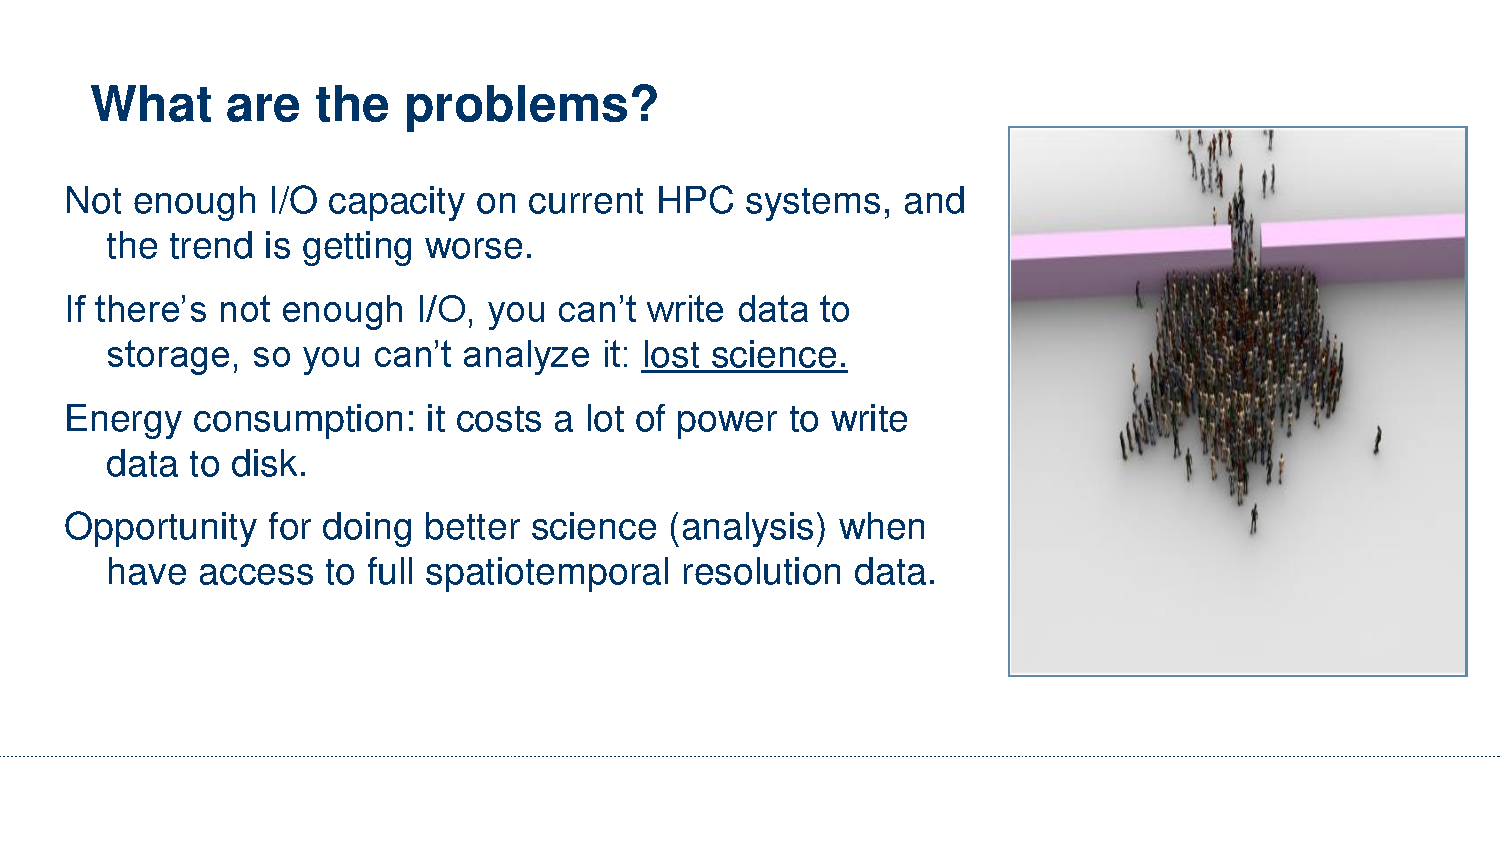
\includegraphics[scale=0.5]{io-probs}
\end{center}

\end{frame}

\begin{frame}[t]{Challenges in Application I/O}

\begin{itemize}
\setlength\itemsep{0.4cm}

\item Leveraging aggregate communication and I/O bandwidth of clients
    \begin{itemize}
        \item ... but not overwhelming a resource limited I/O system with uncoordinated accesses!
    \end{itemize}

\item Limiting number of files that must be managed
    \begin{itemize}
      \item Also a performance issue
    \end{itemize}

\item Avoiding unnecessary post-processing

\item Often application teams spend so much time on this that they never get any further:
    \begin{itemize}
      \item Interacting with storage through convenient abstractions
%      \item Storing in portable formats
    \end{itemize}

\end{itemize}

Parallel I/O software is available that can address all
of these problems, when used appropriately.

%\begin{center}
%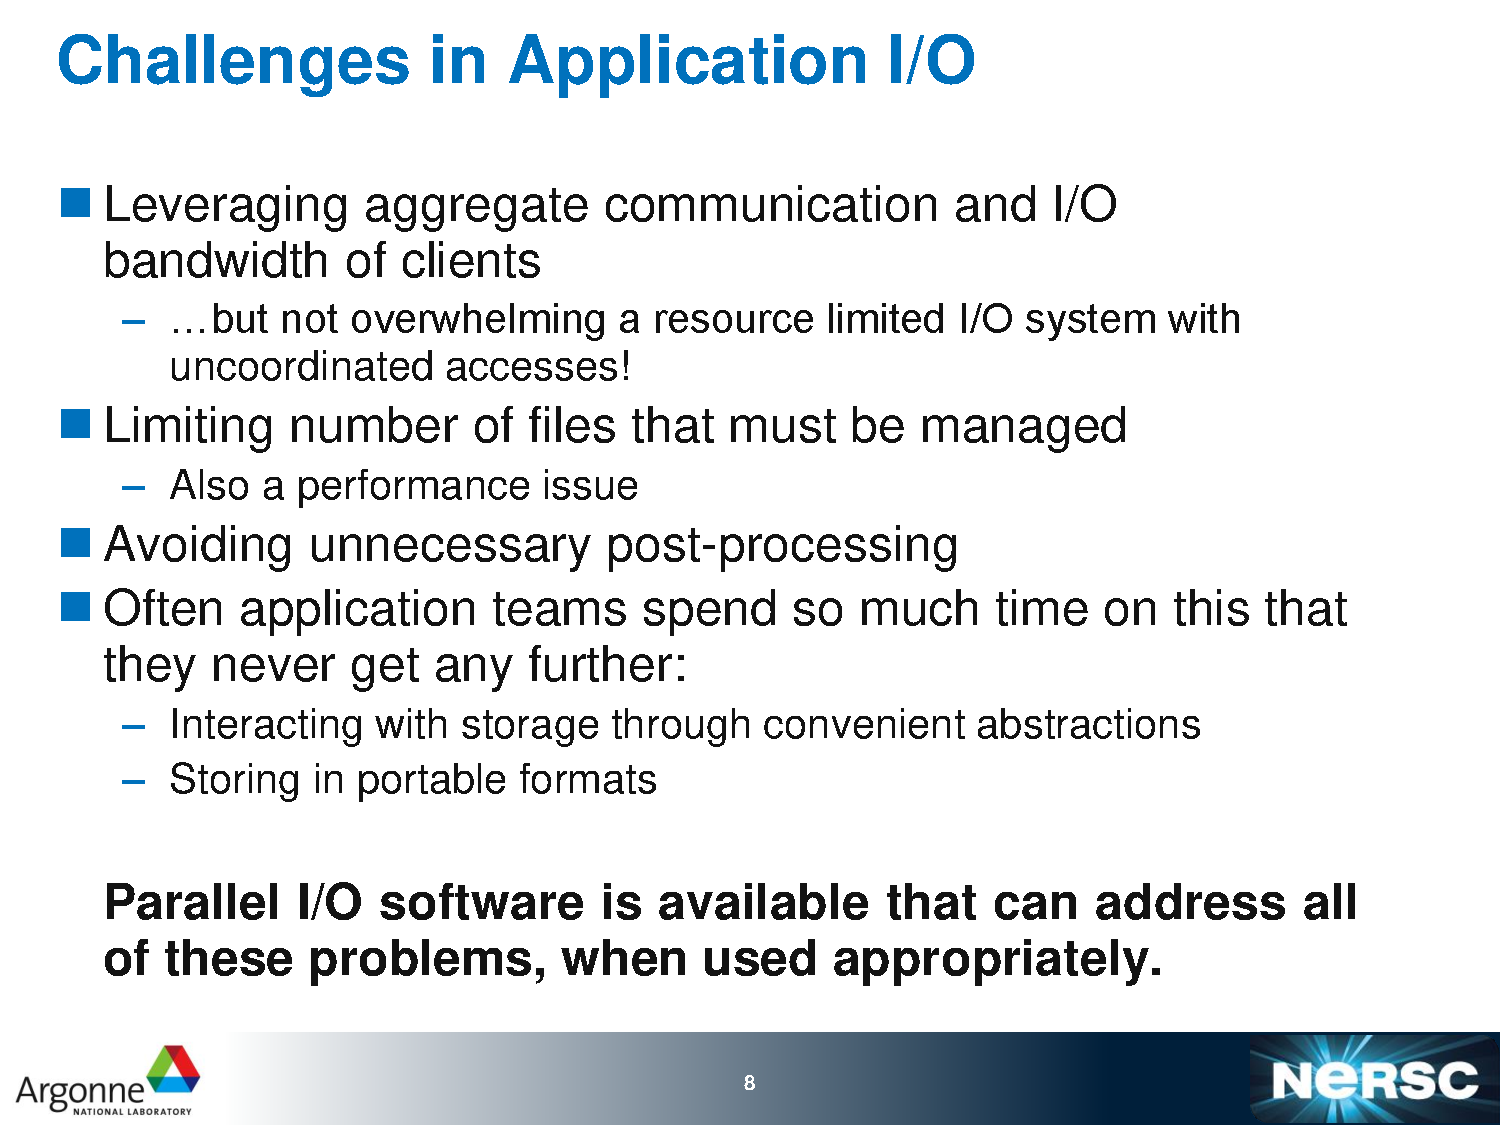
\includegraphics[scale=0.5]{fig/challenges-io}
%\end{center}

\end{frame}

\subsection{Data-driven Research}

\begin{frame}[t]{Data-driven Research}

\begin{itemize}
\setlength\itemsep{1cm}

  \item Data-driven research is the science of letting data tell us what we are looking for.

  \item Database management is the science of efficiently storing and retrieving data.

  \item Data mining is the science of discovering hidden correlations in data.

\end{itemize}

\end{frame}

\begin{frame}[t]{Challenges for Data-driven Research}

\begin{itemize}
\setlength\itemsep{0.4cm}

  \item In HPC, the concerns of storage and computing are traditionally separated and optimised independently from each other and the needs of the end-to-end user.

  \item Workflows composed of data, computing, and communication-intensive tasks should drive interfaces and hardware configurations to best support the programming models.

  \item Many processes still require experts. For example, porting a workflow from one system to another still requires adjusting runtime parameters of applications and deciding on how data is managed.

  \item Data-driven workflows may benefit from the explicit and simultaneous use of a locally heterogeneous set of computing and storage technologies.

\end{itemize}

\end{frame}

\section{Middleware}
\sectionIntro

\subsection{Definition}

\begin{frame}[t]{Middleware}

\begin{itemize}
\setlength\itemsep{0.4cm}

  \item Middleware is software occupying a middle position between application programs and operating systems.

  \begin{center}
  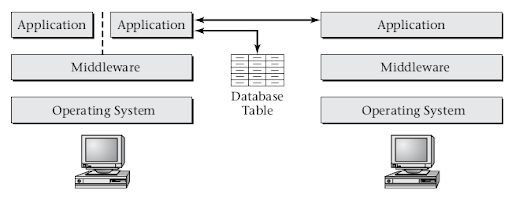
\includegraphics[scale=0.5]{fig/middleware}
  \end{center}

  \item Common middleware examples include database middleware, application server middleware, message-oriented middleware, web middleware, and transaction-processing monitors.

\end{itemize}

\end{frame}

\begin{frame}[t]{Middleware}

\begin{itemize}
\setlength\itemsep{0.4cm}

  \item Middleware is in the middle of the vertical stack, between the application programs and the operating system.

  \item Viewed horizontally rather than vertically, middleware is also in the middle of interactions between different application programs (possibly even running on different computer systems), because it provides mechanisms to support controlled interaction through coordination, persistent storage, naming, and communication.

  \item Relational database systems is one example of middleware.

  \begin{itemize}
    \item Such systems provide a more sophisticated form of persistent storage than the files supported by most operating systems.
  \end{itemize}

\end{itemize}

\end{frame}

\begin{frame}[t]{Describe the role of middleware and file formats}

\begin{itemize}

  \item File formats
    \begin{itemize}
        \item
        \item
    \end{itemize}

  \item
    \begin{itemize}
      \item
    \end{itemize}

\end{itemize}

\end{frame}

\subsection{I/O Solutions}

\begin{frame}[t]{I/O Solutions}

\begin{itemize}

\item As we are moving towards exascale, the gap between computing power and I/O bandwidth will
widen and researchers are looking for solutions to tackle this problem.\\[0.4cm]

\item There are essentially three lines of research:\\[0.4cm]

    \begin{itemize}
    \setlength\itemsep{0.6cm}

      \item at hardware level,
      \item at middleware level,
      \item and at application level.

    \end{itemize}

\end{itemize}

\end{frame}

\begin{frame}[t]{Hardware Level}

\begin{itemize}

    \item Non-volatile memory (NVM)\\[0.4cm]

    \begin{itemize}
    \setlength\itemsep{0.6cm}

        \item Non-volatile memory (NVM) is a type of computer memory that can retrieve stored information even after having been power cycled.

        \item The capabilities of NVM (i.e., capacity, bandwidth, energy consumption) are somewhere in-between main memory and persistent storage, thus it is often used as a ``caching'' solution between these two layers.

        \item Picture

    \end{itemize}

\end{itemize}

\end{frame}

\begin{frame}[t]{Hardware Level}

\begin{itemize}

    \item Burst buffer (BB)\\[0.4cm]

      \begin{itemize}
      \setlength\itemsep{0.6cm}

      \item Burst buffer (BB) is a fast and intermediate storage layer positioned between the front-end computing processes and the back-end storage systems.

      \item HPC applications often show bursty I/O behavior (i.e., all processes read/write at the same time) and burst buffers help to absorb these workloads.

      \item Picture

      \end{itemize}

\end{itemize}

\end{frame}

\begin{frame}[t]{Hardware Level}

\begin{itemize}

      \item Multi-layer Storage Hierarchy (Examples)\\[0.4cm]

        \begin{itemize}
        \setlength\itemsep{0.6cm}

        \item Attached SSDs to compute nodes to aggregate many small I/O requests into few larger ones and/or to compute nodes to speed-up MPI-IO.

        \item Multi-layer storage hierarchy with NVM, SSDs, and different types of hard disks. % drives.

        \item Picture

        \end{itemize}

\end{itemize}

\end{frame}

\begin{frame}[t]{Middleware Level}

\begin{itemize}
\setlength\itemsep{0.4cm}

\item Solutions in I/O middleware.

    \begin{itemize}

    \item E.g., file systems, I/O interfaces.

    \end{itemize}

\item Software framework that overlaps computation and I/O operations by dedicating a single core to I/O tasks.

\item I/O abstraction framework for HPC applications that enables switching between different I/O transport methods with little modification to application code.

\item File systems that improves the scalability of file systems by letting compute nodes manage metadata instead of a centralized server.

\end{itemize}

\end{frame}

\begin{frame}[t]{Application Level}

\begin{itemize}

\item In-situ analysis\\[0.4cm]

    \begin{itemize}
    \setlength\itemsep{0.6cm}

    \item In biology and biomedical engineering, in situ means to examine the phenomenon exactly in place where it occurs (i.e., without moving it to some special medium).

    \item Rather than applications writing their raw output to storage to later be read again for post-processing (e.g., visualization, filtering, statistics), in-situ processing removes this overhead by performing the analysis directly on the same machines as where the applications run.

    \item ParaView, Dax, and Damaris/Viz are tools for large-scale in-situ visualization.

    \end{itemize}

\end{itemize}

\end{frame}

\begin{frame}[t]{Discussion}

\begin{itemize}

\item Mismatch between the massive computational performance of processors and relatively limited I/O bandwidth of storage systems.

\item Three methods to alleviate this problem: new hardware technology, new I/O middleware, and application-specific solutions).

\item Hardware technology shows promising solutions, but different systems might employ different solutions, reducing the portability and increasing the complexity. % of software.

\item Middleware can alleviate some of this complexity with solutions such as ADIOS.

\item In-situ analysis is an example of how application-specific solutions can be used to improve I/O throughput and thus application performance.

\item No one-size-fits-all solution to the storage problem and programmers must take I/O into careful consideration when developing applications.

\end{itemize}

\end{frame}

\section{Performance}
\sectionIntro

\subsection{}

\begin{frame}[t]{I/O Path}

The I/O path describes all the layers (and components) involved in I/O and how they interact.
In brief, the I/O path of a write operation can be described as follows:

    \begin{itemize}

        \item When an application issues an I/O call, data is copied between the user-space buffer and the page cache that is offered in kernel-space.

        \item In kernel-space memory the data is cached and write operations can be deferred as long as free memory is available.

        \item At this point the write call can complete, because a programmer cannot modify kernel-space directly.

        \item A scheduler inside the kernel decides when modified pages are transferred to the block device.

        \item The mapping from offsets in logical files to addresses on the block storage is managed by a file system. Further, file systems provide the hierarchical namespace and offer additional management features.

    \end{itemize}

\end{frame}

\begin{frame}[t]{I/O Performance}

\begin{itemize}
\setlength\itemsep{0.6cm}

  \item There are several aspects involved in delivering high I/O performance to parallel applications, from hardware characteristics to methods that manipulate workloads to improve achievable performance.

  \item Running the same application with different I/O configurations gives the possibility to tune the I/O system according to the application access pattern.

  \item One way to predict application performance in HPC systems with different I/O configurations is by using modelling and simulation techniques.

\end{itemize}

\end{frame}

\begin{frame}[t]{I/O Layers}

\begin{center}
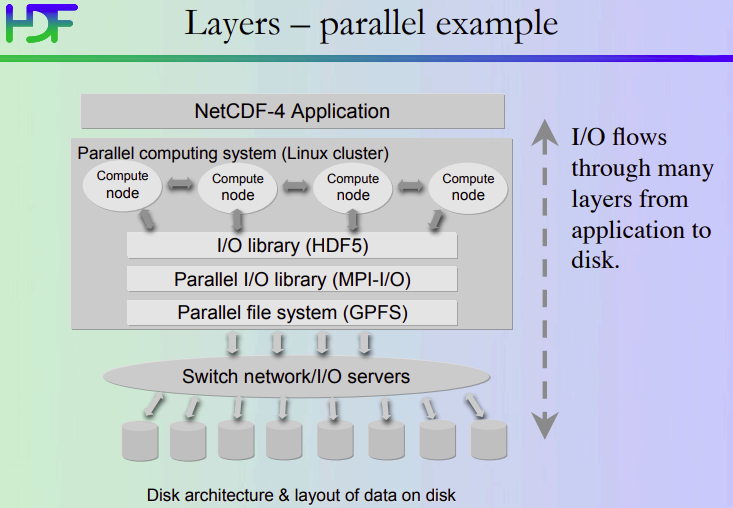
\includegraphics[scale=0.5]{fig/io-layers}
\end{center}

\end{frame}

\begin{frame}[t]{I/O Stack}

\begin{center}
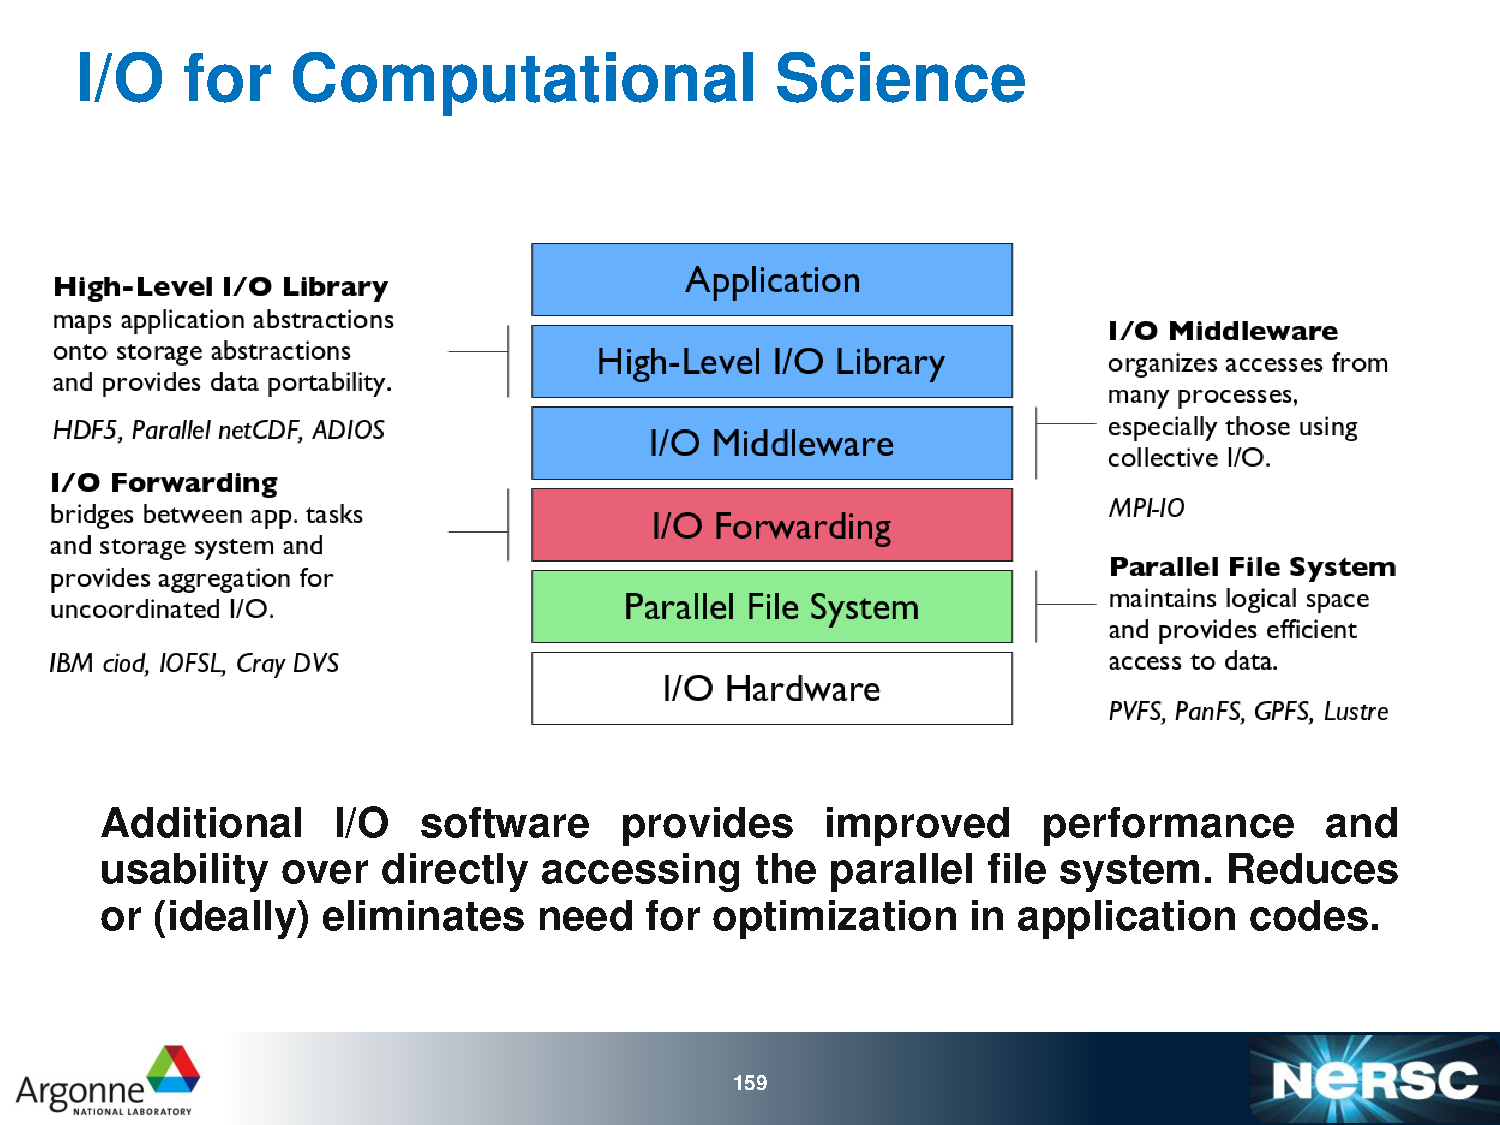
\includegraphics[scale=0.5]{fig/io-stack2}
\end{center}

\end{frame}

\begin{frame}[t]{I/O Stack}

\begin{center}
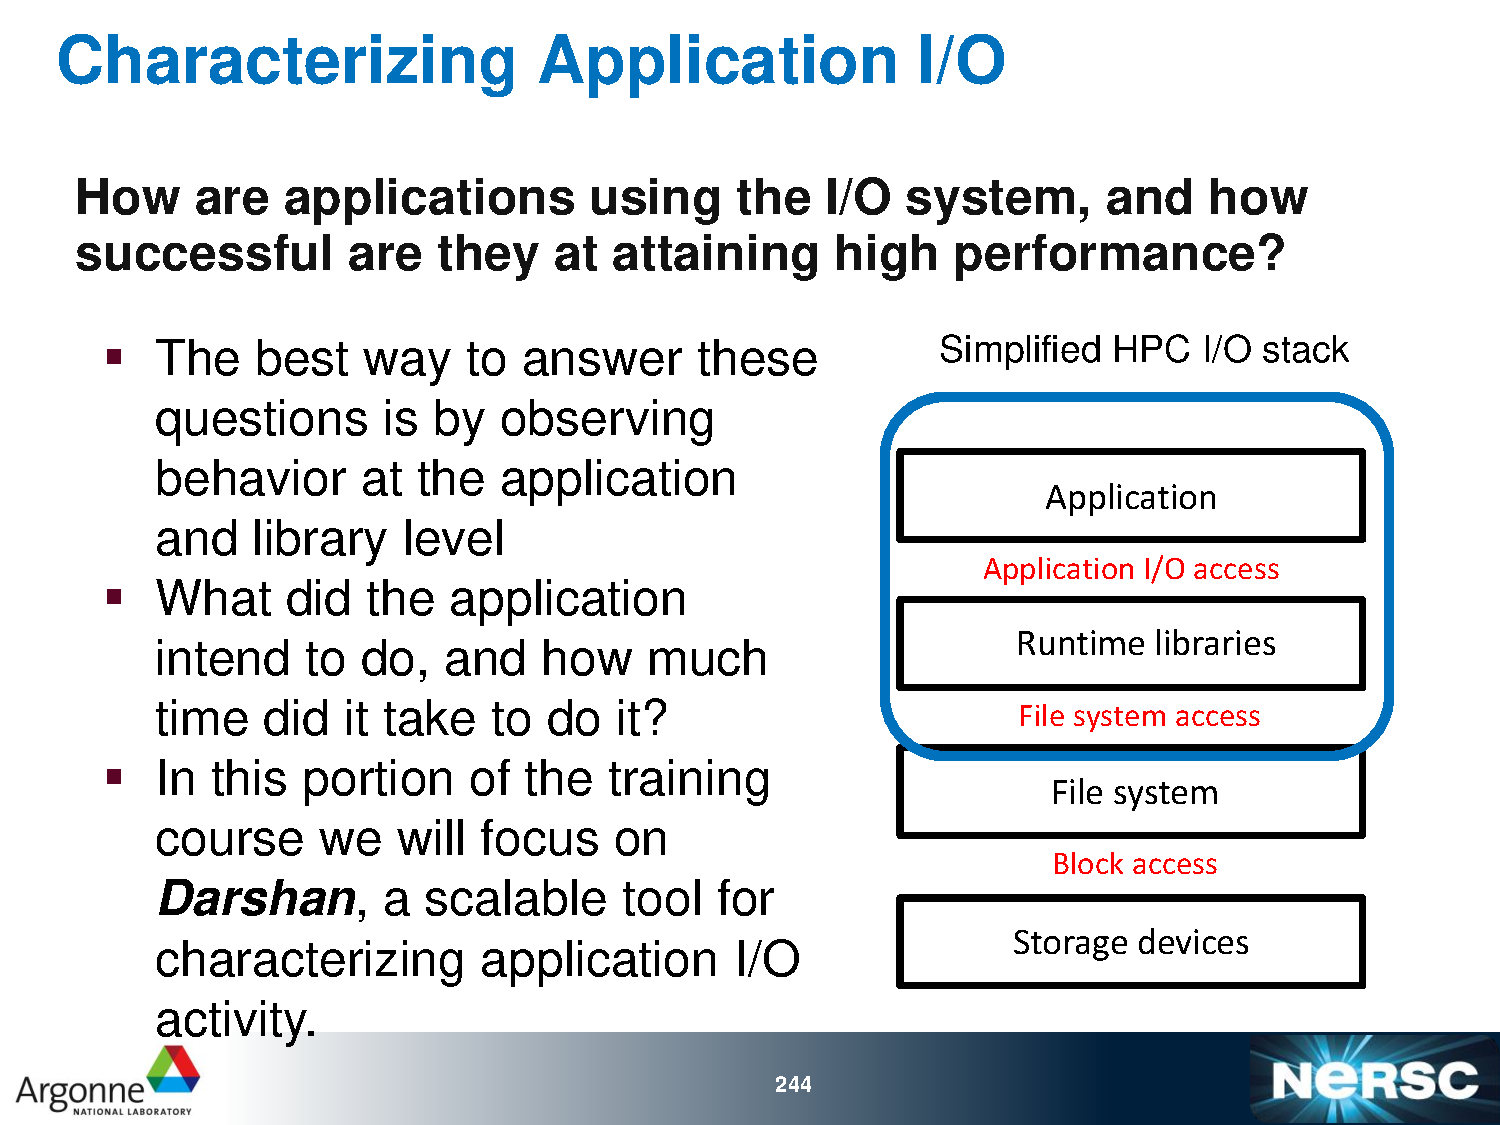
\includegraphics[scale=0.3]{fig/io-stack3}
\end{center}

\end{frame}

\begin{frame}[t]{Storage Stack}

\begin{center}
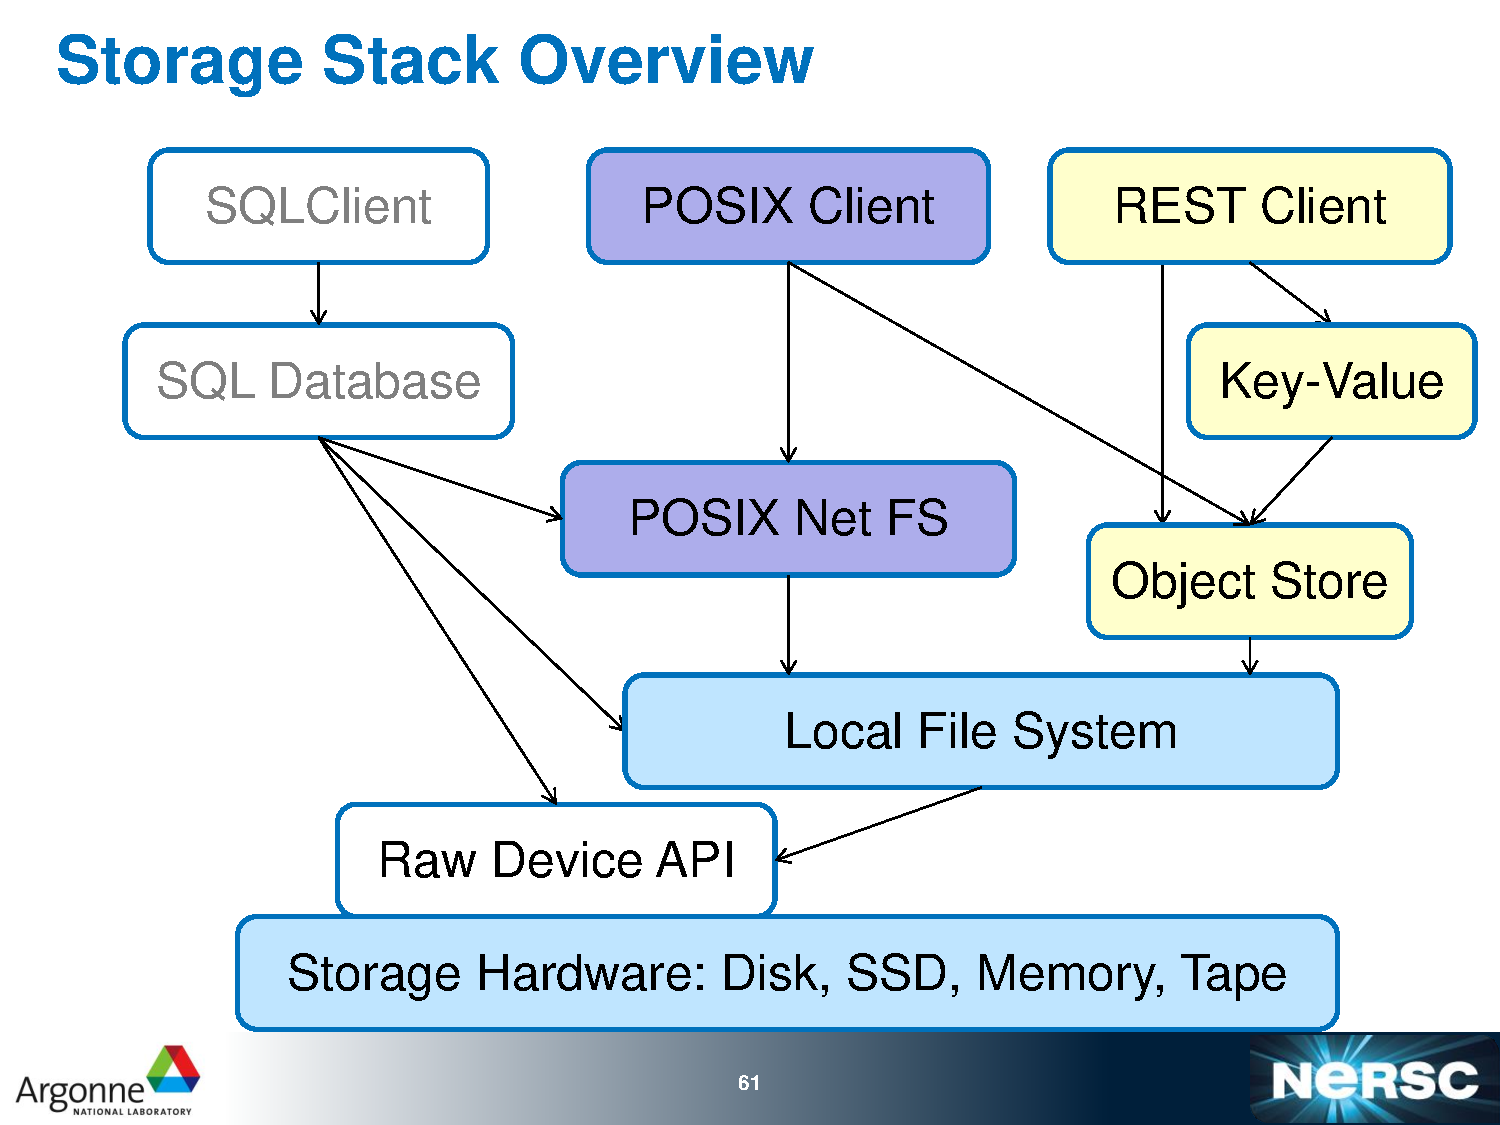
\includegraphics[scale=0.3]{fig/storage-stack}
\end{center}

\end{frame}

\begin{frame}[t]{Storage Stack}

\begin{center}
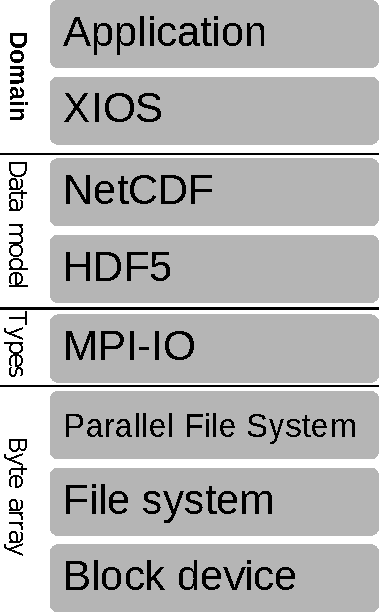
\includegraphics[scale=0.5]{fig/layers-xios}
\end{center}

\end{frame}

\begin{frame}[t]{Typical I/O Performance Issues}

 Access patterns:

    \begin{itemize}
    \setlength\itemsep{0.3cm}
        \item Access granularity
        \item Randomness
        \item Concurrency
        \item Load balance
        \item Access type
        \item Predictability
    \end{itemize}

\end{frame}

\begin{frame}[t]{Typical I/O Performance Issues}

I/O strategy:

    \begin{itemize}
    \setlength\itemsep{0.3cm}
        \item Caching algorithm
        \item Replication
        \item High availability (HA) support
        \item I/O forwarding
        \item Aggregation
        \item Scheduling
    \end{itemize}

\end{frame}

\begin{frame}[t]{Typical I/O Performance Issues}

Parallel file system:

    \begin{itemize}
    \setlength\itemsep{0.3cm}
        \item Design
        \item Implementation
        \item Resource consumption
        \item Communication
        \item Data distribution
        \item Metadata handling
        \item Consistency semantics
        \item Locking strategy
    \end{itemize}

\end{frame}

\begin{frame}[t]{Assess and Optimize the Application I/O Performance}

\begin{itemize}
\setlength\itemsep{0.4cm}

\item Develop general considerations about what influences the I/O performance

\begin{itemize}
  \item What?
\end{itemize}

\item Analyze access pattern and define how it defines the performance of the I/O subsystems

\begin{itemize}
  \item How?
\end{itemize}

\item Apply I/O strategies to improve the access pattern

\begin{itemize}
  \item Which?
\end{itemize}

\item Identify options for the deployed optimization strategies in a specific parallel file system

\begin{itemize}
  \item Which?
\end{itemize}

\end{itemize}

\end{frame}

\section{Model}
\sectionIntro

\subsection{}

\begin{frame}[t]{I/O Performance Tuning ``Rules of Thumb''}

\begin{center}
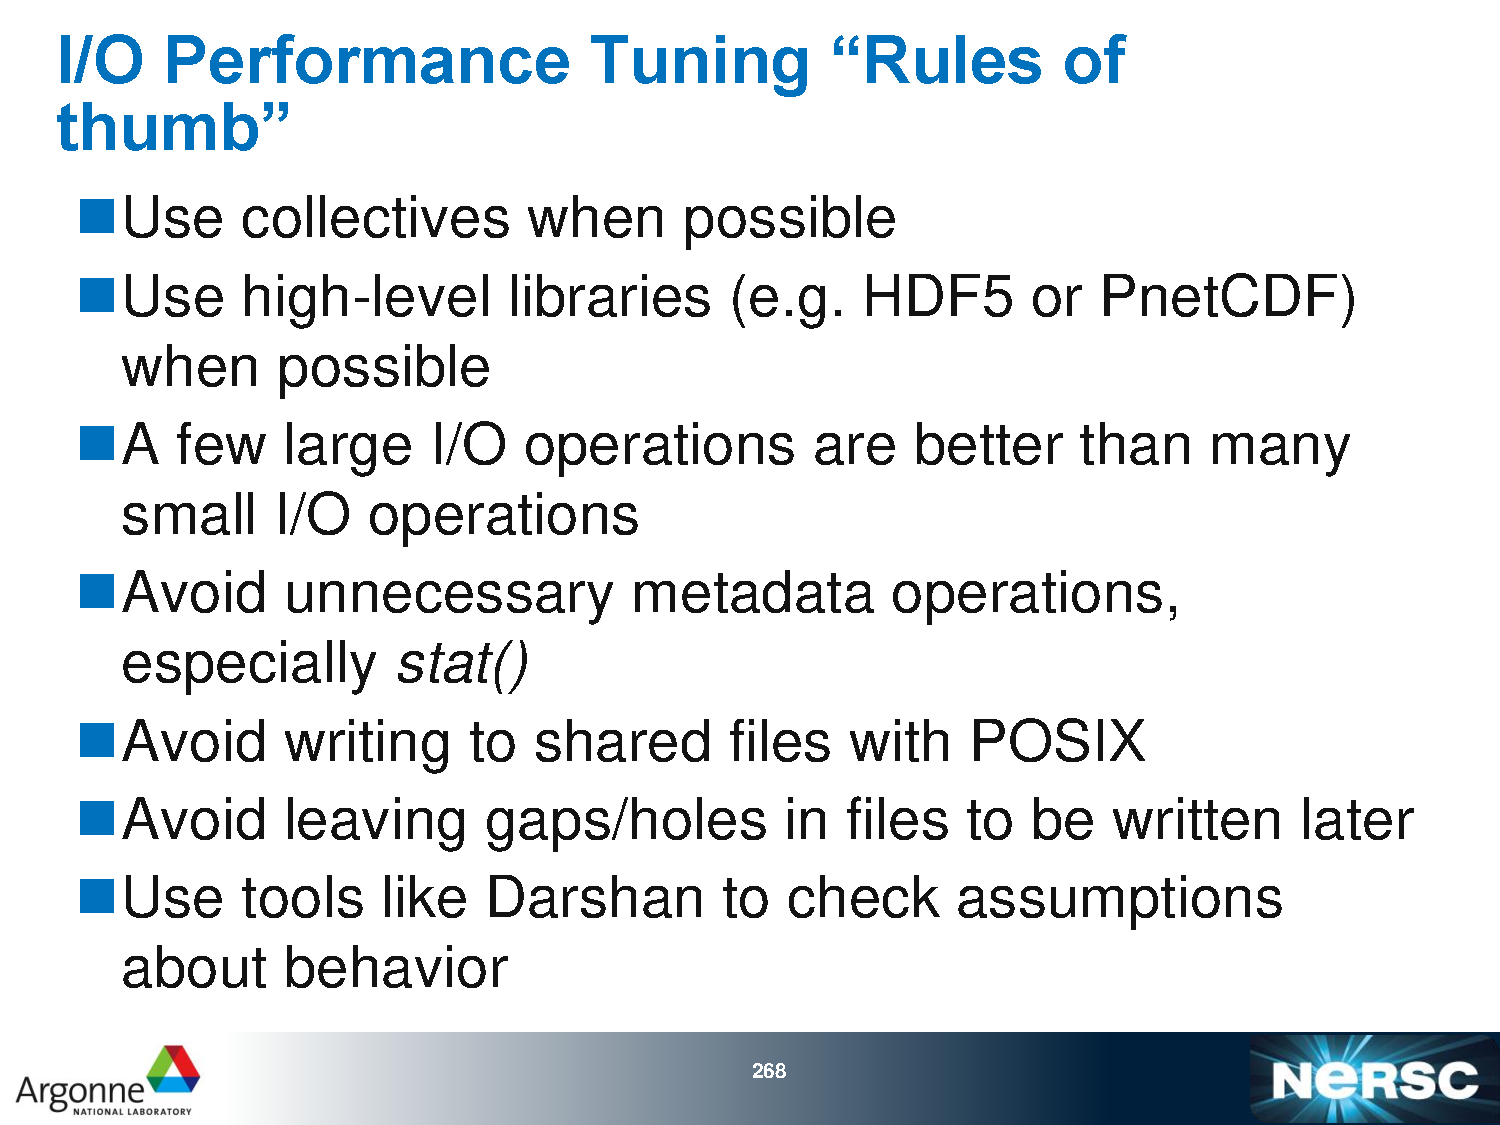
\includegraphics[scale=0.35]{fig/io-rules}
\end{center}

\end{frame}

\begin{frame}[t]{I/O Performance Model}

\begin{center}
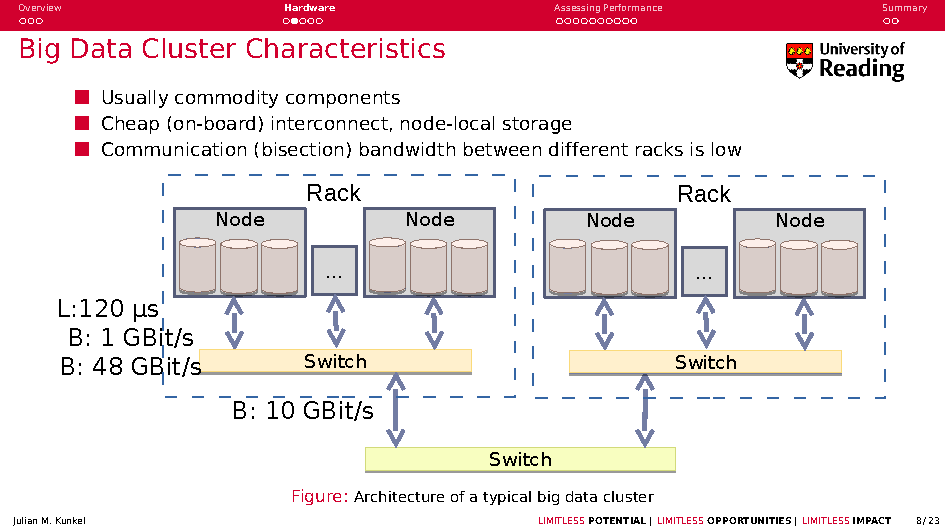
\includegraphics[scale=0.7]{fig/5-1}
\end{center}

\end{frame}

\begin{frame}[t]{I/O Performance Model}

\begin{center}
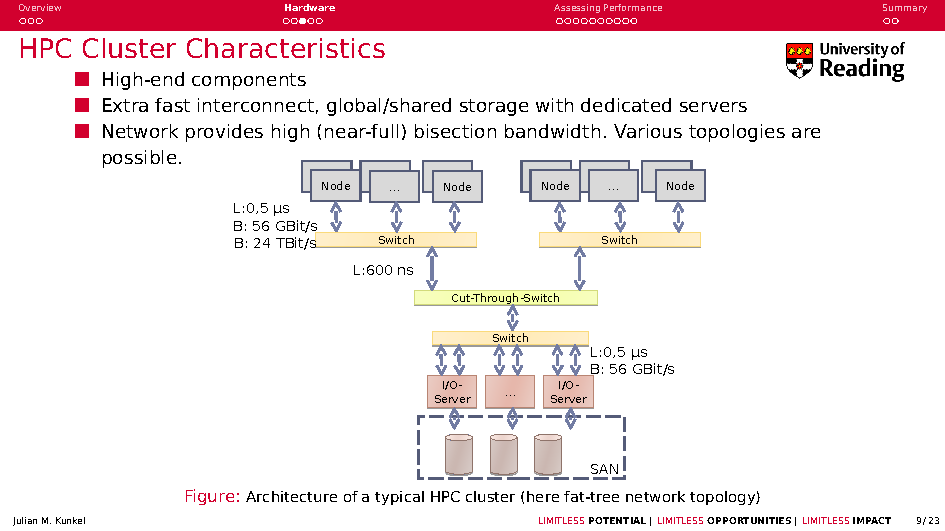
\includegraphics[scale=0.7]{fig/5-2}
\end{center}

\end{frame}

\begin{frame}[t]{I/O Performance Model}

\begin{center}
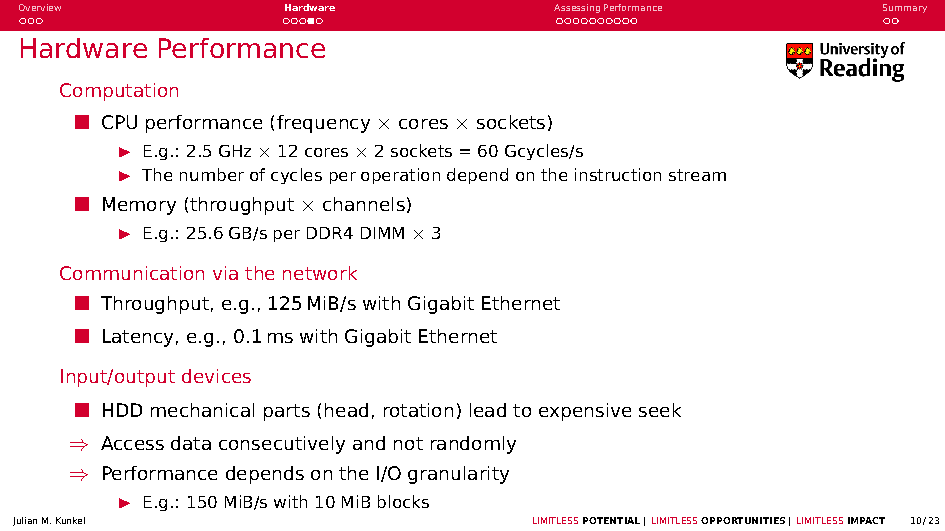
\includegraphics[scale=0.7]{fig/5-3}
\end{center}

\end{frame}

\begin{frame}[t]{I/O Performance Model}

\begin{center}
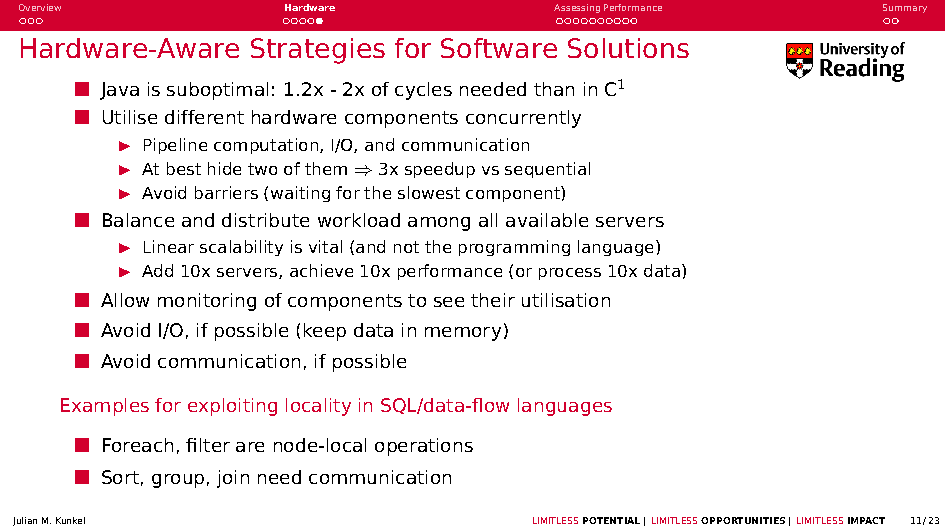
\includegraphics[scale=0.7]{fig/5-4}
\end{center}

\end{frame}

\begin{frame}[t]{I/O Performance Model}

\begin{center}
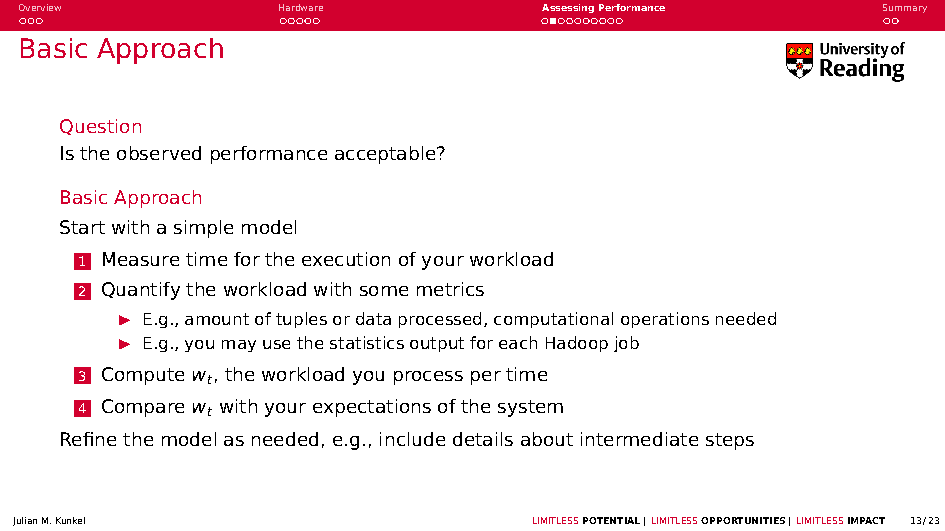
\includegraphics[scale=0.7]{fig/5-5}
\end{center}

\end{frame}

\begin{frame}[t]{I/O Performance Model}

\begin{center}
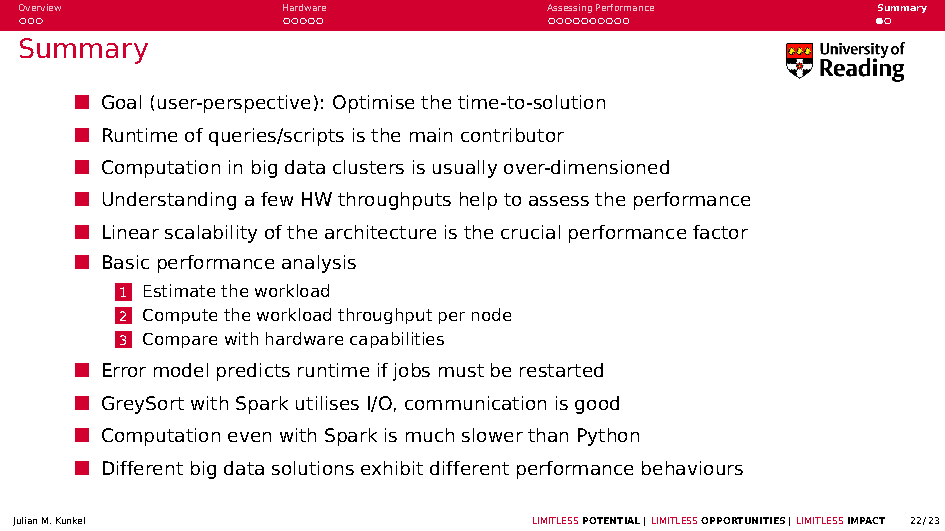
\includegraphics[scale=0.7]{fig/5-6}
\end{center}

\end{frame}

\section{NetCDF}
\sectionIntro

\subsection{}

\begin{frame}[t]{NetCDF}

\begin{itemize}
\setlength\itemsep{0.4cm}

\item In a simple view, NetCDF is:

    \begin{itemize}
        \item A data mode.
        \item A file format.
        \item A set of APIs and libraries for various programming languages.
    \end{itemize}

\item Together, the data model, file format, and APIs support the creation, access, and sharing of scientific data.

\item NetCDF allows the user to describe multidimensional data and include metadata which further characterizes the data.

\item NetCDF APIs are available for most programming languages used in geosciences.

\end{itemize}

\end{frame}

\begin{frame}[fragile]{Common Data form Language (CDL)}

\begin{itemize}
\setlength\itemsep{0.3cm}

\item The notation used to describe a NetCDF object is called CDL (network Common Data form Language), which provides a convenient way of describing NetCDF datasets.

\begin{center}
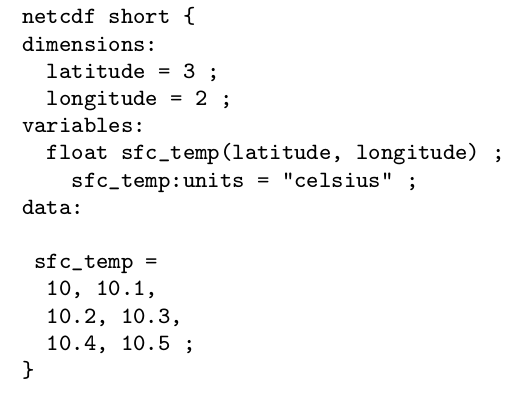
\includegraphics[scale=0.4]{fig/short-nc}\vspace{-0.2cm}
\end{center}

\begin{comment}

\tiny{

\begin{verbatim}

netcdf short {
dimensions:
  latitude = 3 ;
  longitude = 2 ;
variables:
  float sfc_temp(latitude, longitude) ;
    sfc_temp:units = "celsius" ;
data:

 sfc_temp =
  10, 10.1,
  10.2, 10.3,
  10.4, 10.5 ;
}

\end{verbatim}

}

\end{comment}

\item The NetCDF system includes utilities for producing human-oriented CDL text files from binary NetCDF datasets and vice-versa.

\end{itemize}

\end{frame}

\begin{frame}[t]{The Classic NetCDF Model}

\begin{itemize}

\item A NetCDF file (dataset) has a path name and possibly some dimensions, variables, global (file-level) attributes, and data values associated with the variables.

\end{itemize}

\begin{center}
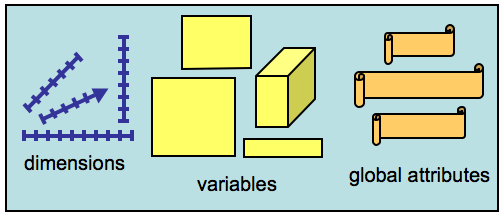
\includegraphics[scale=0.6]{fig/netcdf-classic}
\end{center}

\end{frame}

\begin{frame}[t]{NetCDF Data Models}

    \begin{itemize}

        \item Classic: Simplest model -- Dimensions, variables, attributes

        \item Enhanced: More powerful model -- Adds groups, types, nesting

    \end{itemize}

    \begin{center}
    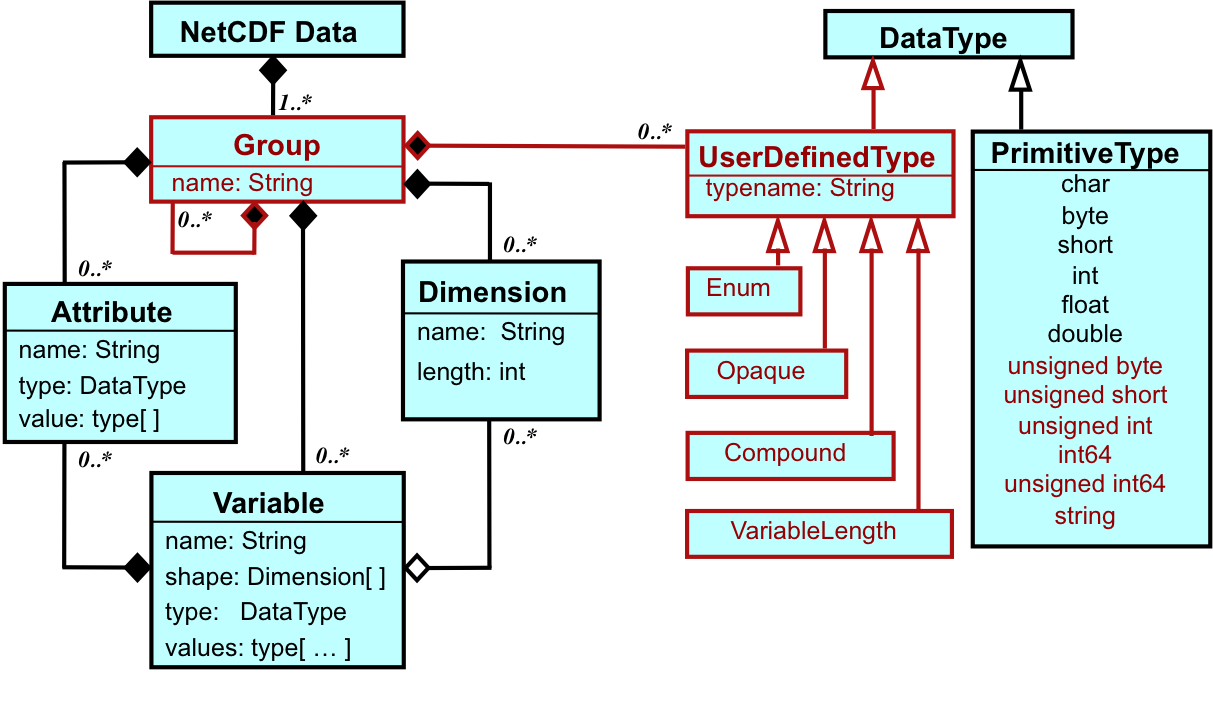
\includegraphics[scale=0.5]{fig/nc4-uml}
    \end{center}

\end{frame}

\begin{frame}[t]{The NetCDF-4 Enhanced Data Model}

\begin{itemize}
\setlength\itemsep{0.4cm}

    \item The NetCDF-4 Enhanced Data Model, which is known as the ``Common Data Model'', is part of an effort of Unidata to find a common engineering language for the development of scientific data solutions.

    \item The model contains the variables, dimensions, and attributes of the classic data model, but adds:

    \begin{itemize}

        \item Groups -- A way of hierarchically organizing data, similar to directories in a Unix file system.\\[0.2cm]

        \item User-defined types -- The user can now define compound types (like C structures), enumeration types, variable length arrays, and opaque types.

    \end{itemize}

\end{itemize}

\end{frame}

\begin{frame}[t]{The NetCDF-4 Enhanced Data Model}

    \begin{itemize}
    \setlength\itemsep{0.4cm}
        \item A file has a top-level unnamed group.
        \item Each group may contain one or more named subgroups, user-defined types, variables, dimensions, and attributes.
        \item Variables also have attributes.
        \item Variables may share dimensions, indicating a common grid.
        \item One or more dimensions may be of unlimited length.
    \end{itemize}

\end{frame}

\begin{frame}[t]{NetCDF-4 and HDF5}

NetCDF-4 uses HDF5 as a storage layer:

\begin{itemize}
\setlength\itemsep{0.4cm}

    \item Provide performance advantages of HDF5
    \item Compression
    \item Chunking
    \item Efficient schema changes
    \item Useful for very large or complex data
    \item Suitable for high-performance computing

\end{itemize}

\end{frame}

\begin{frame}[t]{NetCDF Data Model}

\begin{center}
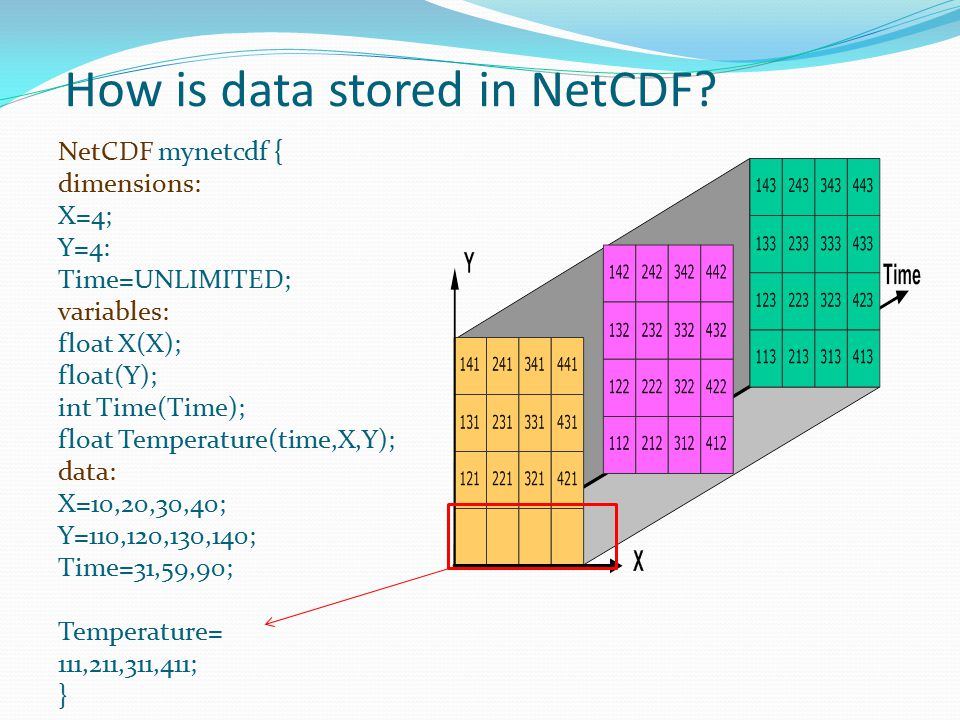
\includegraphics[scale=0.4]{fig/netcdf-data}
\end{center}

\end{frame}

\begin{frame}[t]{HDF5 Data Model}

\begin{center}
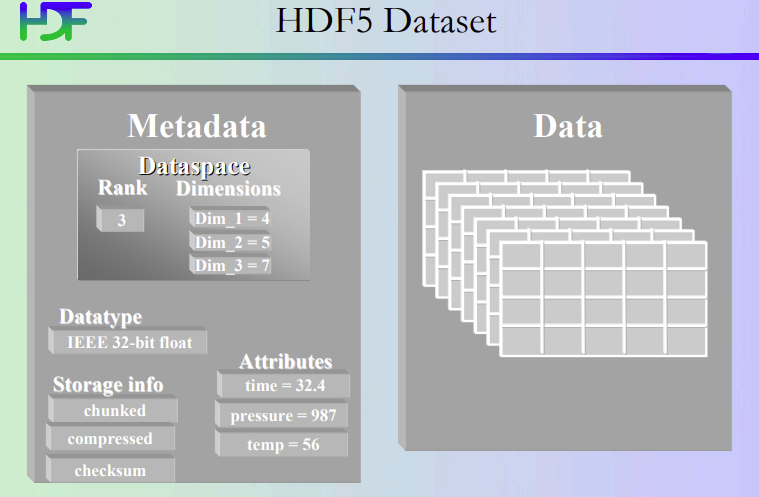
\includegraphics[scale=0.5]{fig/hdf5-data}
\end{center}

\end{frame}

\begin{frame}[t]{ESDM Data Model}

\begin{center}
% \includegraphics[scale=0.4]{fig/esdm-data}
\end{center}

\end{frame}

\begin{frame}[t]{Experience-based ``Best Practices'' for Writing NetCDF Files}

    \begin{itemize}
    \setlength\itemsep{0.3cm}

        \item	Conventions
        \begin{itemize}
          \item Developers should be familiar with and use existing NetCDF conventions.
        \end{itemize}

        \item	Coordinate Systems
        \begin{itemize}
          \item Spatial and temporal location of data are supported by use of coordinate systems.
        \end{itemize}

        \item	Variable Grouping
        \begin{itemize}
          \item How you group data into variables can determine whether common analysis and visualization software can effectively use the data.
        \end{itemize}

        \item	Variable Attributes
        \begin{itemize}
          \item Conventional variable attributes supply necessary metadata.
        \end{itemize}

    \end{itemize}

\end{frame}

\begin{frame}[t]{Experience-based ``Best Practices'' for Writing NetCDF Files}

    \begin{itemize}
    \setlength\itemsep{0.4cm}

        \item	Strings and Character Variables
        \begin{itemize}
          \item Use character data properly for representing text strings.
        \end{itemize}

        \item Calendar Date and Time
        \begin{itemize}
          \item Represent calendar dates and times with standards and conventions.
        \end{itemize}

        \item	Packed Data Values
        \begin{itemize}
          \item Conventions for packing numeric data to save space have some subtleties.
        \end{itemize}

        \item Missing Data Values
        \begin{itemize}
          \item To indicate that data values are missing, invalid, or not written, special values are conventionally used.
        \end{itemize}

    \end{itemize}

\end{frame}

\begin{frame}[t]{Climate and Forecast (CF) Conventions}

\begin{itemize}
\setlength\itemsep{0.3cm}

\item The Climate and Forecast (CF) conventions are metadata conventions for earth science data, intended to promote the processing and sharing of files created with the NetCDF API.

% \item The CF conventions define metadata that are included in the same file as the data (thus making the file ``self-describing'').

\item The purpose of the CF conventions is to require conforming datasets to contain sufficient metadata that they are self-describing:

    \begin{itemize}

      \item Each variable in the file has an associated description of what it represents, including physical units if appropriate.

      \item Each value can be located in space (relative to earth-based coordinates) and time.

    \end{itemize}

\item The CF conventions enable users of data from different sources to decide which data are comparable and allows building applications with powerful extraction, regridding, and display capabilities.

\end{itemize}

\end{frame}

\section{Storage}
\sectionIntro

\subsection{}

\begin{frame}[t]{Describe ongoing research activities in high-performance storage}

\begin{itemize}

  \item
    \begin{itemize}
        \item TODO
        \item
    \end{itemize}
  \item
    \begin{itemize}
      \item
    \end{itemize}
\end{itemize}

\end{frame}


\section{Others}

\begin{frame}[t]{Previous Learning Objectives}

\begin{itemize}

    \item Describe the general layers involved in I/O on a supercomputer
    \item Analyse the implications of parallel I/O on application efficiency
    \item Identify typical I/O performance issues and their causes
    \item Design a data model for NetCDF/CF
    \item Read, analyse, and write NetCDF files in a metadata-aware manner
    \item Visualise and regrid field constructs within NetCDF

\end{itemize}

\end{frame}

\acknowledgement

\end{document}
